\documentclass{article}

\usepackage{xcolor}
\usepackage{hyperref}
\definecolor{COLOR_MEAN}{HTML}{f0f0f0}
\definecolor{LINK_COLOR}{HTML}{636EFA}
\hypersetup{
	colorlinks=true,
	linkcolor=LINK_COLOR,
	urlcolor=LINK_COLOR,
	citecolor=LINK_COLOR,
}

% if you need to pass options to natbib, use, e.g.:
%     \PassOptionsToPackage{numbers, compress}{natbib}
% before loading neurips_2024


% ready for submission
%\usepackage{neurips_2024}


% to compile a preprint version, e.g., for submission to arXiv, add add the
% [preprint] option:
% \usepackage[preprint]{neurips_2024}


% to compile a camera-ready version, add the [final] option, e.g.:
\usepackage[final]{neurips_2024}


% to avoid loading the natbib package, add option nonatbib:
%    \usepackage[nonatbib]{neurips_2024}


\usepackage[utf8]{inputenc} % allow utf-8 input
\usepackage[T1]{fontenc}    % use 8-bit T1 fonts
\usepackage{hyperref}       % hyperlinks
% \usepackage{url}            % simple URL typesetting
\usepackage{xurl}
\usepackage{booktabs}       % professional-quality tables
\usepackage{amsfonts}       % blackboard math symbols
\usepackage{nicefrac}       % compact symbols for 1/2, etc.
\usepackage{microtype}      % microtypography
\usepackage[dvipsnames]{xcolor}         % colors
\usepackage{tabularx}
\usepackage{booktabs}
\usepackage{amsmath}
\usepackage{xspace}
\usepackage{cleveref}
\usepackage{multirow}
\usepackage{multicol}
\usepackage{subcaption}

\usepackage{algorithm} 
\usepackage{algpseudocode}
\usepackage{mathrsfs}
\usepackage{tikz}
\usepackage{listings}
\usepackage{bbm}

\usepackage[symbol]{footmisc}
\definecolor{ntured}{HTML}{D71440}
\hypersetup{
    colorlinks=true,     
    urlcolor=ntured,
}

\lstset{ 
  language=python,                     % the language of the code
  basicstyle=\ttfamily, % the size of the fonts that are used for the code
  numbers=left,                   % where to put the line-numbers
  numberstyle=\tiny\color{Blue},  % the style that is used for the line-numbers
  stepnumber=1,                   % the step between two line-numbers. If it is 1, each line
                                  % will be numbered
  numbersep=5pt,                  % how far the line-numbers are from the code
  backgroundcolor=\color{white},  % choose the background color. You must add \usepackage{color}
  showspaces=false,               % show spaces adding particular underscores
  showstringspaces=false,         % underline spaces within strings
  showtabs=false,                 % show tabs within strings adding particular underscores
  frame=single,                   % adds a frame around the code
  rulecolor=\color{black},        % if not set, the frame-color may be changed on line-breaks within not-black text (e.g. commens (green here))
  tabsize=2,                      % sets default tabsize to 2 spaces
  captionpos=b,                   % sets the caption-position to bottom
  breaklines=true,                % sets automatic line breaking
  breakatwhitespace=false,        % sets if automatic breaks should only happen at whitespace
  keywordstyle=\color{RoyalBlue},      % keyword style
  commentstyle=\color{YellowGreen},   % comment style
  stringstyle=\color{ForestGreen}      % string literal style
} 




% \title{SC3020 Project 1}


% The \author macro works with any number of authors. There are two commands
% used to separate the names and addresses of multiple authors: \And and \AND.
%
% Using \And between authors leaves it to LaTeX to determine where to break the
% lines. Using \AND forces a line break at that point. So, if LaTeX puts 3 of 4
% authors names on the first line, and the last on the second line, try using
% \AND instead of \And before the third author name.


% \author{
% }

\usepackage{graphicx}

\begin{document}
	
\begin{titlepage}
	\begin{figure}[!t]
		\centering
		
\includegraphics[width = 4.3in]{title/logo.pdf}
	\end{figure}
	
	\centering
	\huge{\textbf{SC4002 Natural Language Processing}}\\[0.2in]
	\huge{\textbf{Group Project}}\\[2in]
	
	%	\LARGE{\textbf{YOUR NAME}}\\
	%	\normalsize{Matriculation number}\\[0.2in]
	
	\begin{table}[h]
		\centering
		\resizebox{\textwidth}{!}{%
			\begin{tabular}{lll}
				\toprule
				\textbf{Name} & \textbf{Email} & \textbf{Matric Number} \\
				\midrule
				Pu Fanyi & \texttt{FPU001@e.ntu.edu.sg} & \texttt{U2220175K} \\
				Shan Yi & \texttt{SH0005YI@e.ntu.edu.sg} & \texttt{U2222846C}\\
                Zhang Kaichen & \texttt{ZHAN0564@e.ntu.edu.sg} & \texttt{U2123722J} \\
                Zhang Jiahua & \texttt{jzhang132@e.ntu.edu.sg} & \texttt{U2221393K} \\
                Tang Yutong & \texttt{TANG0513@e.ntu.edu.sg} & \texttt{U2220495H}\\
                Zeng Ruixiao & \texttt{ZENG0146@e.ntu.edu.sg} & \texttt{U2220375D}\\
				\bottomrule
			\end{tabular}%
		}
	\end{table}

	
	
    
	
	%	\large{A Final Year Report submitted to Asian School of the Environment, Nanyang Technological University in partial fulfilment of the requirements for the Degree of }\\[0.1in]
	
	\vspace{0.5in}
	\LARGE{Nanyang Technological University, Singapore}\\[0.3in]
	
	
	\LARGE{2024/2025 Semester 1}
	\newpage
\end{titlepage}
	
% \maketitle

% \begin{abstract}
%     lalala
% \end{abstract}

\section{Introduction}
This report focuses on building and evaluating a sentiment classification system using pretrained word embeddings. Our work is organized into three main parts:

In section 2, we prepare and analyze the word embeddings that form the foundation of our classification system. We use GloVe as our embedding method and address the out-of-vocabulary (OOV) issue through a novel greedy matching approach.

In section 3, we implement and evaluate a basic RNN model for sentiment classification. We explore different strategies for sentence representation and conduct extensive hyperparameter tuning to optimize model performance.

In the last section, we utilized different methods to improve classificat model and proposed our final method.

\paragraph{Note} Results may fluctuate due to variations in settings such as GPU type and other parameters. However, we ensure consistency within each set of ablations and experiments by maintaining identical settings throughout. Specific settings are provided for each experiment we conduct.

\section{Preparing Word Embeddings}

\subsection{Tokenizer and Embeddings}

GloVe \cite{pennington2014glove} is used as our embedding method. We selected \texttt{glove.840B.300d}\footnote{Trained on Common Crawl, 840B tokens, 2.2M vocab, cased and 300d vectors, accessed from \url{https://nlp.stanford.edu/data/glove.840B.300d.zip}} as our pretrained embedding model. To easier manage the GloVe model, we pack the model to Hugging Face \cite{wolf2020transformers}.

We tried to take an overview of this dataset. \textsc{Nltk} tokenizer \cite{bird2006nltk} is used to split the word. We report the \textbf{out-of-vocabulary (OOV)} issue in~\cref{tab:word_stats} and found about $0.96\%$ tokens are unknown in the vocabulary.

\begin{table}[ht]
    \centering
    \begin{tabular}{c | c | c}
    \toprule
    \textbf{Words} & \textbf{Count} & \textbf{Percentage}\\
    \midrule
    Known & $182211$ & $99.04\%$\\
    Unknown & $1757$ & $0.96\%$\\
    \midrule
    Total & $183968$ & $100\%$\\
    \bottomrule
    \end{tabular}
    \vspace{1mm}
    \caption{Word count for the training dataset \cite{Pang+Lee:05a}}
    \label{tab:word_stats}
    \vspace{-2mm}
\end{table}


% \begin{lstlisting}
% >>> glove.tokenizer.demo("pneumonoultramicroscopicsilicovolcanoconiosis")
% \end{lstlisting}

% The output is:

% \begin{lstlisting}
% pne | umo | nou | ltr | amic | rosco | pics | ilic | ovo | lca | noc | oni | osis
% \end{lstlisting}

\subsection{Mitigating Out of Vocabulary Limitations}
To address the OOV issue, we employ two approaches for handling various edge cases. \textbf{1)} We predefine the \texttt{<|UNK|>} token and its ID in the tokenizer class to map any unknown character to this token. The word embedding for \texttt{<|UNK|>} is resized and initialized to zeros. \textbf{2)} To maximize the pretrained knowledge from Glove, we use a \textbf{Greedy Matching} approach, which tokenizes each sentence by breaking down unknown words into recognizable segments. This allows us to reconstruct unknown words using known prefixes, suffixes, and semantic tokens, effectively leveraging the extensive vocabulary and latent space of the word embeddings.

% \begin{lstlisting}
% class Tokenizer(object):
%     def __init__(self, tokenizer_path: str, pad_side: str = "right"):
%         self.unk_token: str = "<|UNK|>"
%         self.unk_id: int = len(self.tokenizer_dict)
% \end{lstlisting}

Then we use the greedy matching algorithm to find the longest matching known word. If an unknown word is encountered, replace it with the \texttt{<|UNK|>} token ID.

There are 2 methods implementing this greedy idea, \textit{Hash-based Greedy Matching} and \textit{Trie-based Greedy Matching}, we analysed both and selected the best one.

\paragraph{Hash-based Greedy Matching} All known words are organised in a hash table $\mathcal{H}$. We enumerate all possible substrings and choose the longest one in $\mathcal{H}$. The detailed algorithm is shown in Algorithm \ref{alg:HashBasedGreedyMatching}. We can proof that the time complexity of this algorithm is at most $\mathcal{O}\left(\|s\|^2\right)$. If we define the average word length is $\mathcal{W}$, the average time complexity is

\begin{equation}
\begin{aligned}
T(s, \mathcal{W}) &= \mathbb{E}\left[\sum_{i=1}^{\|s\|}\mathbbm{1}_{s_i\text{ is beginning of a word}}\cdot (\|s\| - i)\right]\\
&=\sum_{i=1}^{\|s\|}(\|s\| - i)\cdot\mathbb{P}(s_i\text{ is beginning of a word})\\
&=\mathcal{O}\left(\frac{\|s\|^2}{\mathcal{W}}\right)
\end{aligned}
\end{equation}

\paragraph{Trie-based Greedy Matching} Algorithm \ref{alg:TrieBasedGreedyMatching} illustrates implementing the greedy matching algorithm with Trie \cite{de1959file}. In this algorithm, every character in $s$ will only be visited at once, so the time complexity is $\mathcal{O}(\|s\|)$.

Although Trie-based Greedy Matching shows a better time complexity, we found that in \cite{Pang+Lee:05a}, $\|s\|$ is always small as there is no long contexts, while building a Trie costs extra spaces and time. So we finally decided to adopt Hash-based Greedy Matching for our algorithm. The code snip is listed in Appendix \ref{appendix:greedy_matching}.

\begin{algorithm}
	\caption{\textsc{TrieBasedGreedyMatching}}
    \label{alg:HashBasedGreedyMatching}
	\begin{algorithmic}
        \State $\mathcal{H} \leftarrow \textsc{BuildHash}(\text{known words})$
        \State $s\leftarrow$ input sentense
        \State $L \leftarrow 0$
        \State $\mathcal{M} \leftarrow$ empty list
        \While {$L < \textsc{Length}(s)$}
            \State $R \leftarrow \emptyset$
            \For{$r \in [L, \textsc{Length}(s))$}
                \State $t\leftarrow \textsc{Strip}(s_{L:r})$
                \If{$t \in \mathcal{H}$}
                    \State $R\leftarrow r$
                \EndIf
            \EndFor
            \State $L\leftarrow R + 1$
            \If {$R = \emptyset$}
            \State $\textsc{Append}(\mathcal{M}, \texttt{<|UNK|>})$
            \Else
            \State $\textsc{Append}(\mathcal{M}, s_{L:R})$
            \EndIf
        \EndWhile
        \State \Return $\mathcal{M}$
	\end{algorithmic} 
\end{algorithm}

\begin{algorithm}
	\caption{\textsc{TrieBasedGreedyMatching}}
    \label{alg:TrieBasedGreedyMatching}
	\begin{algorithmic}
        \State $\mathcal{T} \leftarrow \textsc{BuildTrie}(\text{known words})$
        \State $s\leftarrow$ input sentense
        \State $L \leftarrow 0$
        \State $\mathcal{M} \leftarrow$ empty list
        \While {$L < \textsc{Length}(s)$}
            \While {$L < \textsc{Length}(s) \land \lnot \textsc{Visible}(s_L)$ }
            \State $L\leftarrow L + 1$
            \EndWhile
            \State $R \leftarrow \emptyset$
            \State $n \leftarrow \textsc{Root}(\mathcal{T})$
            \For{$r\in [L, \textsc{Length}(s)) \land \textsc{Son}(n, s_r)\neq \emptyset$}
                \State $n\leftarrow \textsc{Son}(n, s_r)$
                \If {$s_{L:r}$ is a known word}
                    \State $R\leftarrow r$
                \EndIf
            \EndFor
            \State $L\leftarrow R$
            \State $\textsc{Append}(\mathcal{M}, s_{L:R-1})$
            \If {$R = \emptyset$}
            \State $\textsc{Append}(\mathcal{M}, \texttt{<|UNK|>})$
            \Else
            \State $\textsc{Append}(\mathcal{M}, s_{L:R})$
            \EndIf
        \EndWhile
        \State \Return $\mathcal{M}$
	\end{algorithmic} 
\end{algorithm}




\section{RNN}
\label{sec:part-rnn}

\subsection{Model Training}

We utilised \textit{Weights \& Biases Agent}\footnote{Documents available in \url{https://docs.wandb.ai/guides/sweeps}} to track and sweep the best model hyperparameter. Bayesian Optimization \cite{dewancker2016bayesian} is used as the strategy to sweep the best hyperparameter. By default, we set the \textit{require\_grad} for word embedding to False to freeze the parameters. We use the simple RNN design with PyTorch~\citep{paszke2019pytorch} that takes each token as hidden states and iterative to the final token for each sequences.

\subsection{Best model}

Due to computational and time limit, we can only run limited experiments. We employ two search strategies, \textbf{1)} Grid Search, \textbf{2)} Manually tuned. The config and the search space is listed in Table \ref{tab:best_model_config}. However, we find out that one of the config when manually tuned the parameters reaches the best result and we adopt that setting as our best model config

\begin{table}[ht]
    \centering
    \begin{tabular}{c | c | c}
    \toprule
    \textbf{Config} & \textbf{Value} & \textbf{Grid Search Space}\\
    \midrule
    Layer & $5$ & $\{3,4,5,6\}$\\
    Input Dim & $300$ & -\\
    Hidden Dim & $512$ & - \\
    \midrule
    Optimizer & AdamW & - \\
    LR Scheduler & \texttt{CosineAnnealingLR} & - \\
    Warmup Ratio & 0.03 & - \\
    Learning Rate & $1.63\times 10^{-5}$ & $1 \times 10^{-3} \sim 1 \times 10^{-5}$\\
    Weight Decay & $0.4$ & - \\
    Batch Size & $4 \text{ (GPUs)}\times 8$ & $4\times \{8, 16, 32\}$\\
    \bottomrule
    \end{tabular}
    \caption{Best Model Config}
    \label{tab:best_model_config}
\end{table}

We also present our grid search results in~\cref{fig:sweep} for multiple trials and use the best model config that achieve the highest evaluation accuracy.

\begin{figure}[h]
    \centering
    \centering
    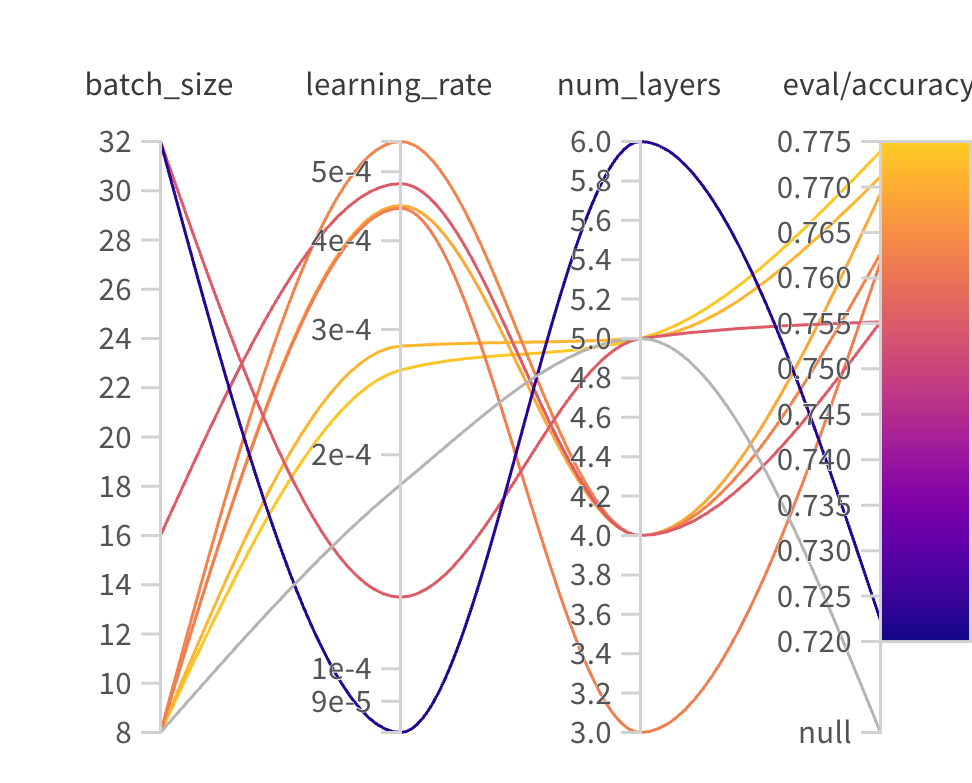
\includegraphics[width=0.85\linewidth]{images/sweep.png}
    \caption{Sweep result}
    \label{fig:sweep}
\end{figure}



\subsection{Model Performance}

\begin{table}[ht]
    \centering
    \begin{tabular}{c | c | c | c}
    \toprule
    \textbf{Metric} & \textbf{Train set} & \textbf{Validation set} & \textbf{Test set}\\
    \midrule
         \textbf{Loss} & $0.5619$ & $0.5228$ & $0.5416$\\
         \textbf{Accuracy} & - & $77.86\%$ & $76.27\%$\\
    \bottomrule
    \end{tabular}
    \caption{Performance table}
    \label{tab:performance}
\end{table}

Our model's performance, as shown in Table~\ref{tab:performance}, is evaluated across the training, validation, and test sets using both loss and accuracy metrics. The loss values are 0.5619, 0.5228, and 0.5416 for the training, validation, and test sets, respectively, indicating consistent performance with slight variations across the datasets. The model achieves an accuracy of 77.86\% on the validation set and 76.27\% on the test set, suggesting that it generalizes well to unseen data with minimal overfitting.

\paragraph{Setting} We use the same settings to run all the experiments with batch size equals to 8 and learning rate equals to $1 \times 10^{-5}$. For every run, we train 10 epochs and report the final validation and test result.

\subsection{Sentence Representation Methods}

\begin{table}[h]
\centering
\caption{The result of using different sentence representation strategies}
\label{tab:sentence}
\begin{tabular}{l|llll}
\toprule
Aggregation & Test/Acc      & Test/Loss     & Val/Acc       & Val/Loss      \\
\midrule
Average     & 0.72          & 0.63          & 0.73          & 0.63          \\
Sum         & \textbf{0.76} & \textbf{0.56} & \textbf{0.76} & \textbf{0.55} \\
Final Token & 0.51          & 0.69          & 0.50          & 0.69         
\end{tabular}
\end{table}

We compare three sentence representation methods—average, sum, and final token—using accuracy and loss metrics on both the validation and test sets. As shown in Table~\ref{tab:sentence}, the sum aggregation method achieves the best performance, with a test accuracy of 0.76 and a test loss of 0.56. This method also yields a validation accuracy of 0.76 and a validation loss of 0.55, outperforming both the average and final token methods. The average method yields moderate results, with a test accuracy of 0.72 and validation accuracy of 0.73, while the final token method shows the lowest performance across all metrics. These results indicate that summing embeddings captures sentence information most effectively in our RNN model, supporting our decision to use this method as the default aggregation strategy.



\section{Enhancement}
\subsection{Unfreezing the word embedding}

As the models we used above are based on the froze pre-trained word embedding which is trained with general corpus, this word embedding may not perform the best on our current corpus. In this section, we will unfreeze the word embedding so that it can better match our current corpus.

\begin{table}[h]
\centering
\caption{Result of the Unfreezing Word Embedding}
\label{tab:unfreeze}
\begin{tabular}{l|llll}
\toprule
                & Test/Acc      & Test/Loss     & Val/Acc       & Val/Loss      \\
\midrule
Unfreeze &  77.01 & 53.29 & 78.42 & 51.82
\end{tabular}
\end{table}

\subsection{Mitigating the OOV word influence}

\begin{table}[h]
\centering
\caption{Result of the OOV strategy}
\label{tab:oov}
\begin{tabular}{l|llll}
\toprule
                & Test/Acc      & Test/Loss     & Val/Acc       & Val/Loss      \\
\midrule
Simple Ignore   & 0.71          & 0.61          & \textbf{0.74} & \textbf{0.60} \\
Greedy Matching & \textbf{0.73} & \textbf{0.60} & 0.73          & 0.61         
\end{tabular}
\end{table}

Our approach to mitigating the out-of-vocabulary (OOV) issue is evaluated using two strategies: simple ignore (replacing OOV tokens with a padding token) and a hash-based greedy matching method, implemented in our code as described in~\cref{alg:HashBasedGreedyMatching}. Both strategies were evaluated on accuracy and loss for the validation and test sets under the same experimental conditions, with the word embeddings unfrozen and trained for 3 epochs.

As shown in Table~\ref{tab:oov}, the greedy matching strategy slightly outperforms the simple ignore method on test accuracy (0.73 vs. 0.71) and test loss (0.60 vs. 0.61). However, the simple ignore method achieves marginally better results on the validation set, with a validation accuracy of 0.74 and validation loss of 0.60. These results suggest that while the greedy matching method is generally more effective on the test set. Though simple ignore performs better on the validation set, it is shows trend to overfit on the test set and may perform even worse on more complex dataset.


\subsection{biLSTM and biGRU}

\begin{table}[h]
\centering
\caption{Result of the biLSTM and biGRU}
\label{tab:bilstm}
\begin{tabular}{l|llll}
\toprule
                & Test/Acc      & Test/Loss     & Val/Acc       & Val/Loss      \\
\midrule
biLSTM & 0.77 & 0.53 & 0.79 & 0.52\\
biGRU & 0.78 & 0.53 & 0.78 & 0.52
\end{tabular}
\end{table}

Table~\ref{tab:bilstm} presents the performance results for the biLSTM and biGRU models. The biLSTM achieves a test accuracy of 0.77 with a test loss of 0.53, while its validation accuracy and loss are 0.79 and 0.52, respectively. The biGRU model shows slightly higher test accuracy at 0.78 with the same test loss of 0.53, and its validation accuracy and loss are 0.78 and 0.52, respectively.

\subsection{CNN}

Our CNN model achieves a test accuracy of 0.77 and a test loss of 0.54, with a validation accuracy of 0.77 and validation loss of 0.52, as shown in Table~\ref{tab:cnn}. The hyperparameters were optimized using a WandB agent to ensure the model’s best performance under our experimental conditions.

\begin{table}[h]
\centering
\caption{Result of the CNN}
\label{tab:cnn}
\begin{tabular}{l|llll}
\toprule
                & Test/Acc      & Test/Loss     & Val/Acc       & Val/Loss      \\
\midrule
CNN & 0.77 & 0.54 & 0.77 & 0.52
\end{tabular}
\end{table}

\subsection{Model enhancement}

\begin{table}[bt]
\centering
\caption{The result of our enhancement method}
\label{tab:enhance}
\begin{tabular}{l|llll}
\toprule
         & Test/Acc      & Test/Loss     & Val/Acc       & Val/Loss      \\
\midrule
Baseline & 0.72          & 0.59          & 0.75          & 0.58          \\
w. Attn  & \textbf{0.74} & \textbf{0.57} & \textbf{0.76} & \textbf{0.55}
\end{tabular}
\end{table}

We incorporate a self-attention mechanism prior to the aggregation step to leverage global information from each token, aiming to enhance the model's ability to capture contextual dependencies. The impact of this approach is shown in Table~\ref{tab:enhance}, where we compare the baseline model with and without self-attention.

The model with self-attention (denoted as ‘w. Attn’) outperforms the baseline across both validation and test sets. Specifically, it achieves a test accuracy of 0.74 and a test loss of 0.57, compared to 0.72 and 0.59 for the baseline. On the validation set, the self-attention model yields an accuracy of 0.76 and a loss of 0.55, surpassing the baseline's accuracy of 0.75 and loss of 0.58. These results suggest that integrating self-attention enhances the model's performance by effectively capturing token-level interactions, which improves generalization on unseen data.

\subsection{Discussion}

\begin{figure}
    \centering
    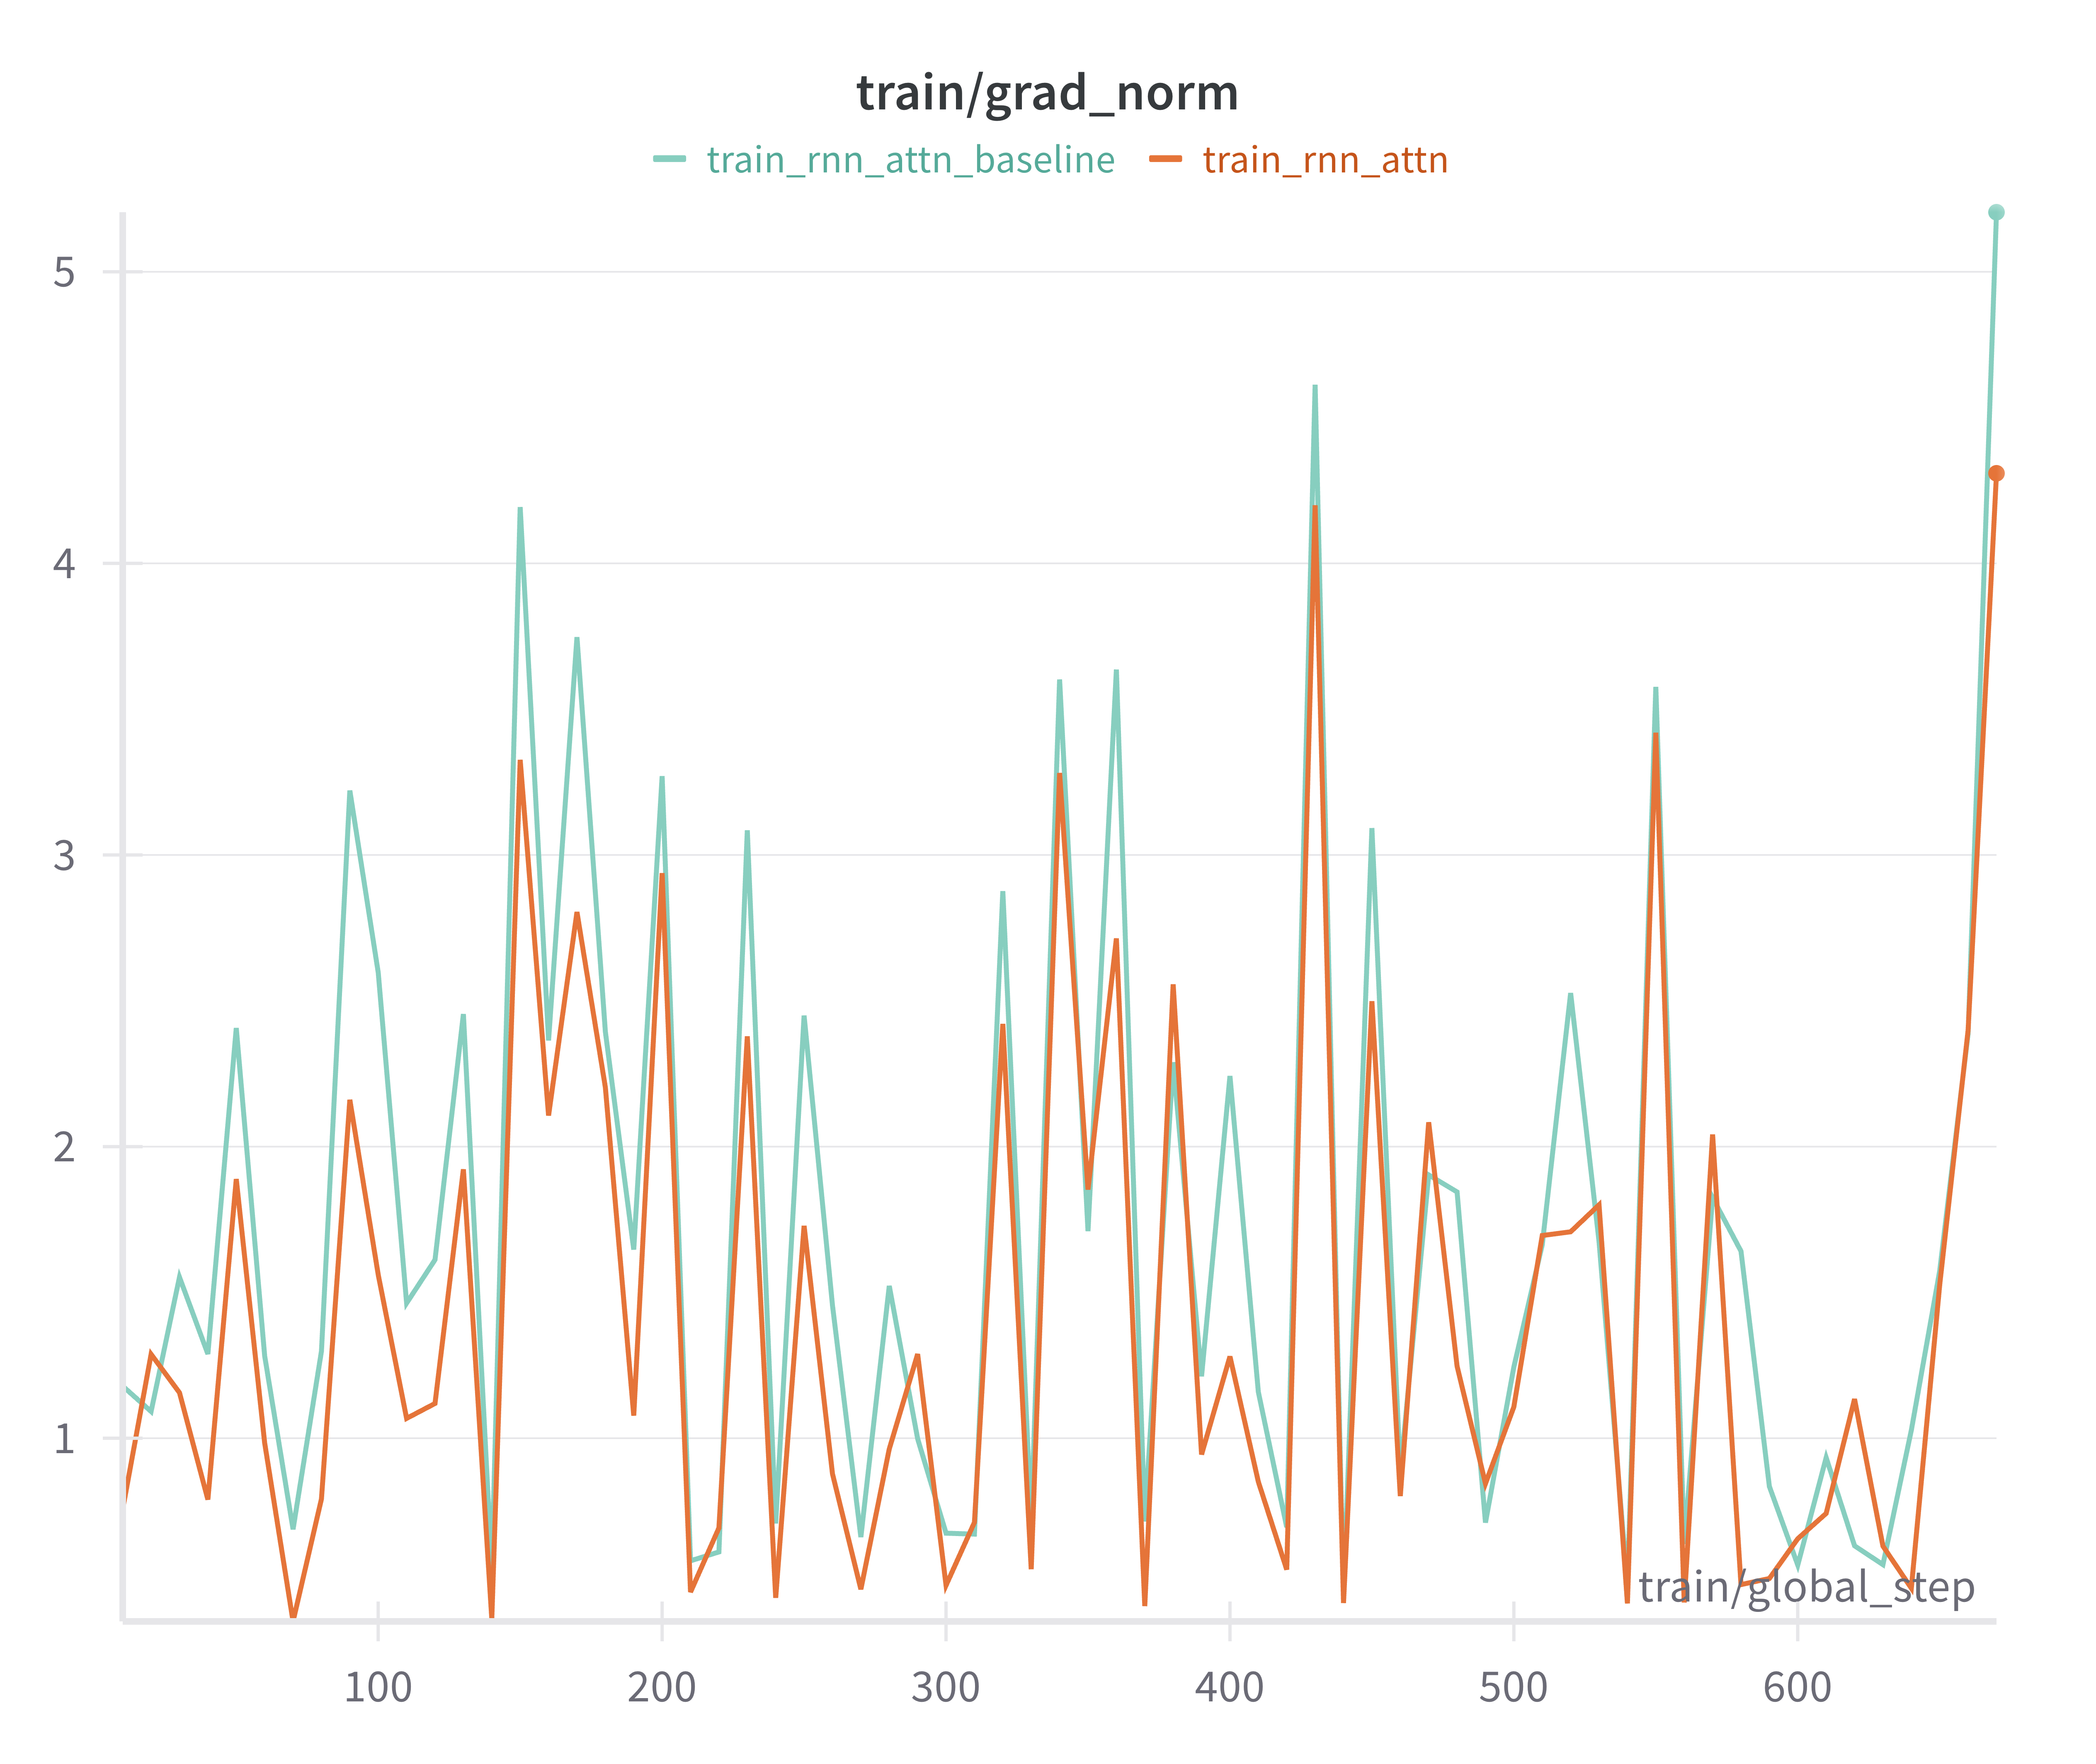
\includegraphics[width=0.75\linewidth]{images/grad_norm.png}
    \caption{A demonstration of the gradient norm in our training process}
    \label{fig:grad-norm}
\end{figure}

In this subsection, we summarize our findings from previous experiments and discuss factors that may have influenced the model's performance.

\paragraph{Vocabulary Size} We believe vocabulary size significantly impacts model performance. In our ablation studies, using a smaller GloVe embedding yielded worse results compared to a larger version under the same settings. With only around 1\% of tokens in the test set facing out-of-vocabulary (OOV) issues, the model can still extract substantial information from the pretrained GloVe vocabulary. Consequently, our strategy for addressing OOV issues provided only minimal improvements.

\paragraph{Dataset Size} The dataset contains approximately 8,000 rows, which limits the distribution from which the model can learn. Even if the model is scaled, without leveraging domain-specific knowledge from large pretrained models such as BERT, training from scratch remains challenging on such a small dataset.

\paragraph{Parameter Tuning} Parameter tuning proved to be particularly impactful with this small dataset. We suspect that due to the limited data distribution, the loss landscape is sharp, making convergence to a stable minimum challenging. An example of the gradient norm using the RNN is shown in~\cref{fig:grad-norm}. As illustrated, the gradient norm fluctuates significantly, indicating large steps taken by the optimizer and highlighting the difficulty of achieving stability

%\input{sections/conclusion}

\newpage

\bibliographystyle{plain} % or another style like apalike, abbrvnat, etc.
\bibliography{references/ref} % assumes you have a references.bib file

\newpage
\appendix

\section{Code for Greedy Matching}\label{appendix:greedy_matching}

\begin{lstlisting}
def greedy_match(self, s: str):
    tokens = []
    i = 0
    while i < len(s):
        longest_match = None
        for j in range(i + 1, len(s) + 1):
            substring = s[i:j]
            if substring.strip() in self.tokenizer_dict:
                if longest_match is None or len(substring) > len(longest_match):
                    longest_match = substring

        if longest_match:
            tokens.append(self.tokenizer_dict[longest_match.strip()])
            i += len(longest_match)
        else:
            i += 1
            tokens.append(len(self.tokenizer_dict))

    return tokens
\end{lstlisting}

\end{document}